\documentclass{beamer}

\usepackage[utf8]{inputenc}
\usepackage[T1]{fontenc}
\usepackage[english]{babel}
\usepackage{lmodern}
\usepackage{color}
\usepackage{fix-cm}
\usepackage{textpos}
\usepackage{eurosym}
\usepackage{multirow}
\usepackage{perpage}

% Redéfinis les marges des tableaux
\let\oldtabular=\tabular
\def\tabular{\small\oldtabular}
\renewcommand{\arraystretch}{1.5}

\usetheme{Warsaw}
\usecolortheme{orchid}

% Permet de réinitialiser les footnote à chaque frame. Nécéssite 2 compilations.
\MakePerPage{footnote}

\setlength{\TPHorizModule}{0.01\textwidth}
\setlength{\TPVertModule}{0.01\textheight}

\setbeamertemplate{navigation symbols}{}

\title[Elon Musk's strategies to not die on earth]{
    How Elon Musk, with his strategies, wants to bring our civilization to the
    next level?
}
\author[HOUDAYER \and KIM \and RUHIER]{
	Benoit HOUDAYER\\
    \and
    Pauline KIM\\
    \and
	Anthony RUHIER
}
\institute[LE84 - UTBM]{
    Business english (LE84) - Université Technologique de Belfort Montbéliard}
\date{January 2016}

\begin{document}

% Permet de masquer le comptage de slides
\bgroup
\makeatletter
\setbeamertemplate{headline}{}
\setbeamertemplate{footline}
{
  \leavevmode%
  \hbox{%
  \begin{beamercolorbox}[wd=.5\paperwidth,ht=2.25ex,dp=1ex,center]{title in head/foot}%
    \usebeamerfont{title in head/foot}\insertshorttitle
  \end{beamercolorbox}%
  \begin{beamercolorbox}[wd=.5\paperwidth,ht=2.25ex,dp=1ex,center]{date in head/foot}%
    \usebeamerfont{date in head/foot}\insertshortdate{}
%    \insertframenumber{} / \inserttotalframenumber\hspace*{2ex}
  \end{beamercolorbox}}%
}
\makeatother

\begin{frame}[noframenumbering]
 	\frametitle{}
	\titlepage
\end{frame}
\egroup

\begin{frame}[noframenumbering,plain]
    I want Iron Man to punch the Hulk here!
	% \begin{textblock}{0}(5,-5)
    %     \center{\includegraphics[width=.7\paperwidth]{images/logo-fsf.eps}}
	% \end{textblock}
\end{frame}

\logo{
\includegraphics[height=1cm]{images/logo-utbm.eps}\hspace*{2em}}


% Ajout du compteur de slides
\expandafter\def\expandafter\insertshorttitle\expandafter{%
      \insertshorttitle\hfill%
      \insertframenumber\,/\,\inserttotalframenumber}

\begin{frame}
	\begin{small}
	\frametitle{Sommaire}
	\tableofcontents
	\end{small}
\end{frame}

\AtBeginSection[]
{
	\begin{small}
	\begin{frame}
		\frametitle{Sommaire}
		\tableofcontents[currentsection]
	\end{frame}
	\end{small}
}


%%%% Includes des sections :
%%%%%%%%%%%%%%%%%%%%%%%%%%%%%%
%
    \section{Global vision}

\subsection{Character sheets}
\begin{frame}
\frametitle{Character sheets}
\begin{itemize}
    \itemsep2em
    \begin{columns}
        \begin{column}{40mm}
        \item South African from a modest family
        \item PhD in applied physics at Stanford
        \item US \${}12.4 billion in 2016
        \end{column}
        \begin{column}{35mm}
        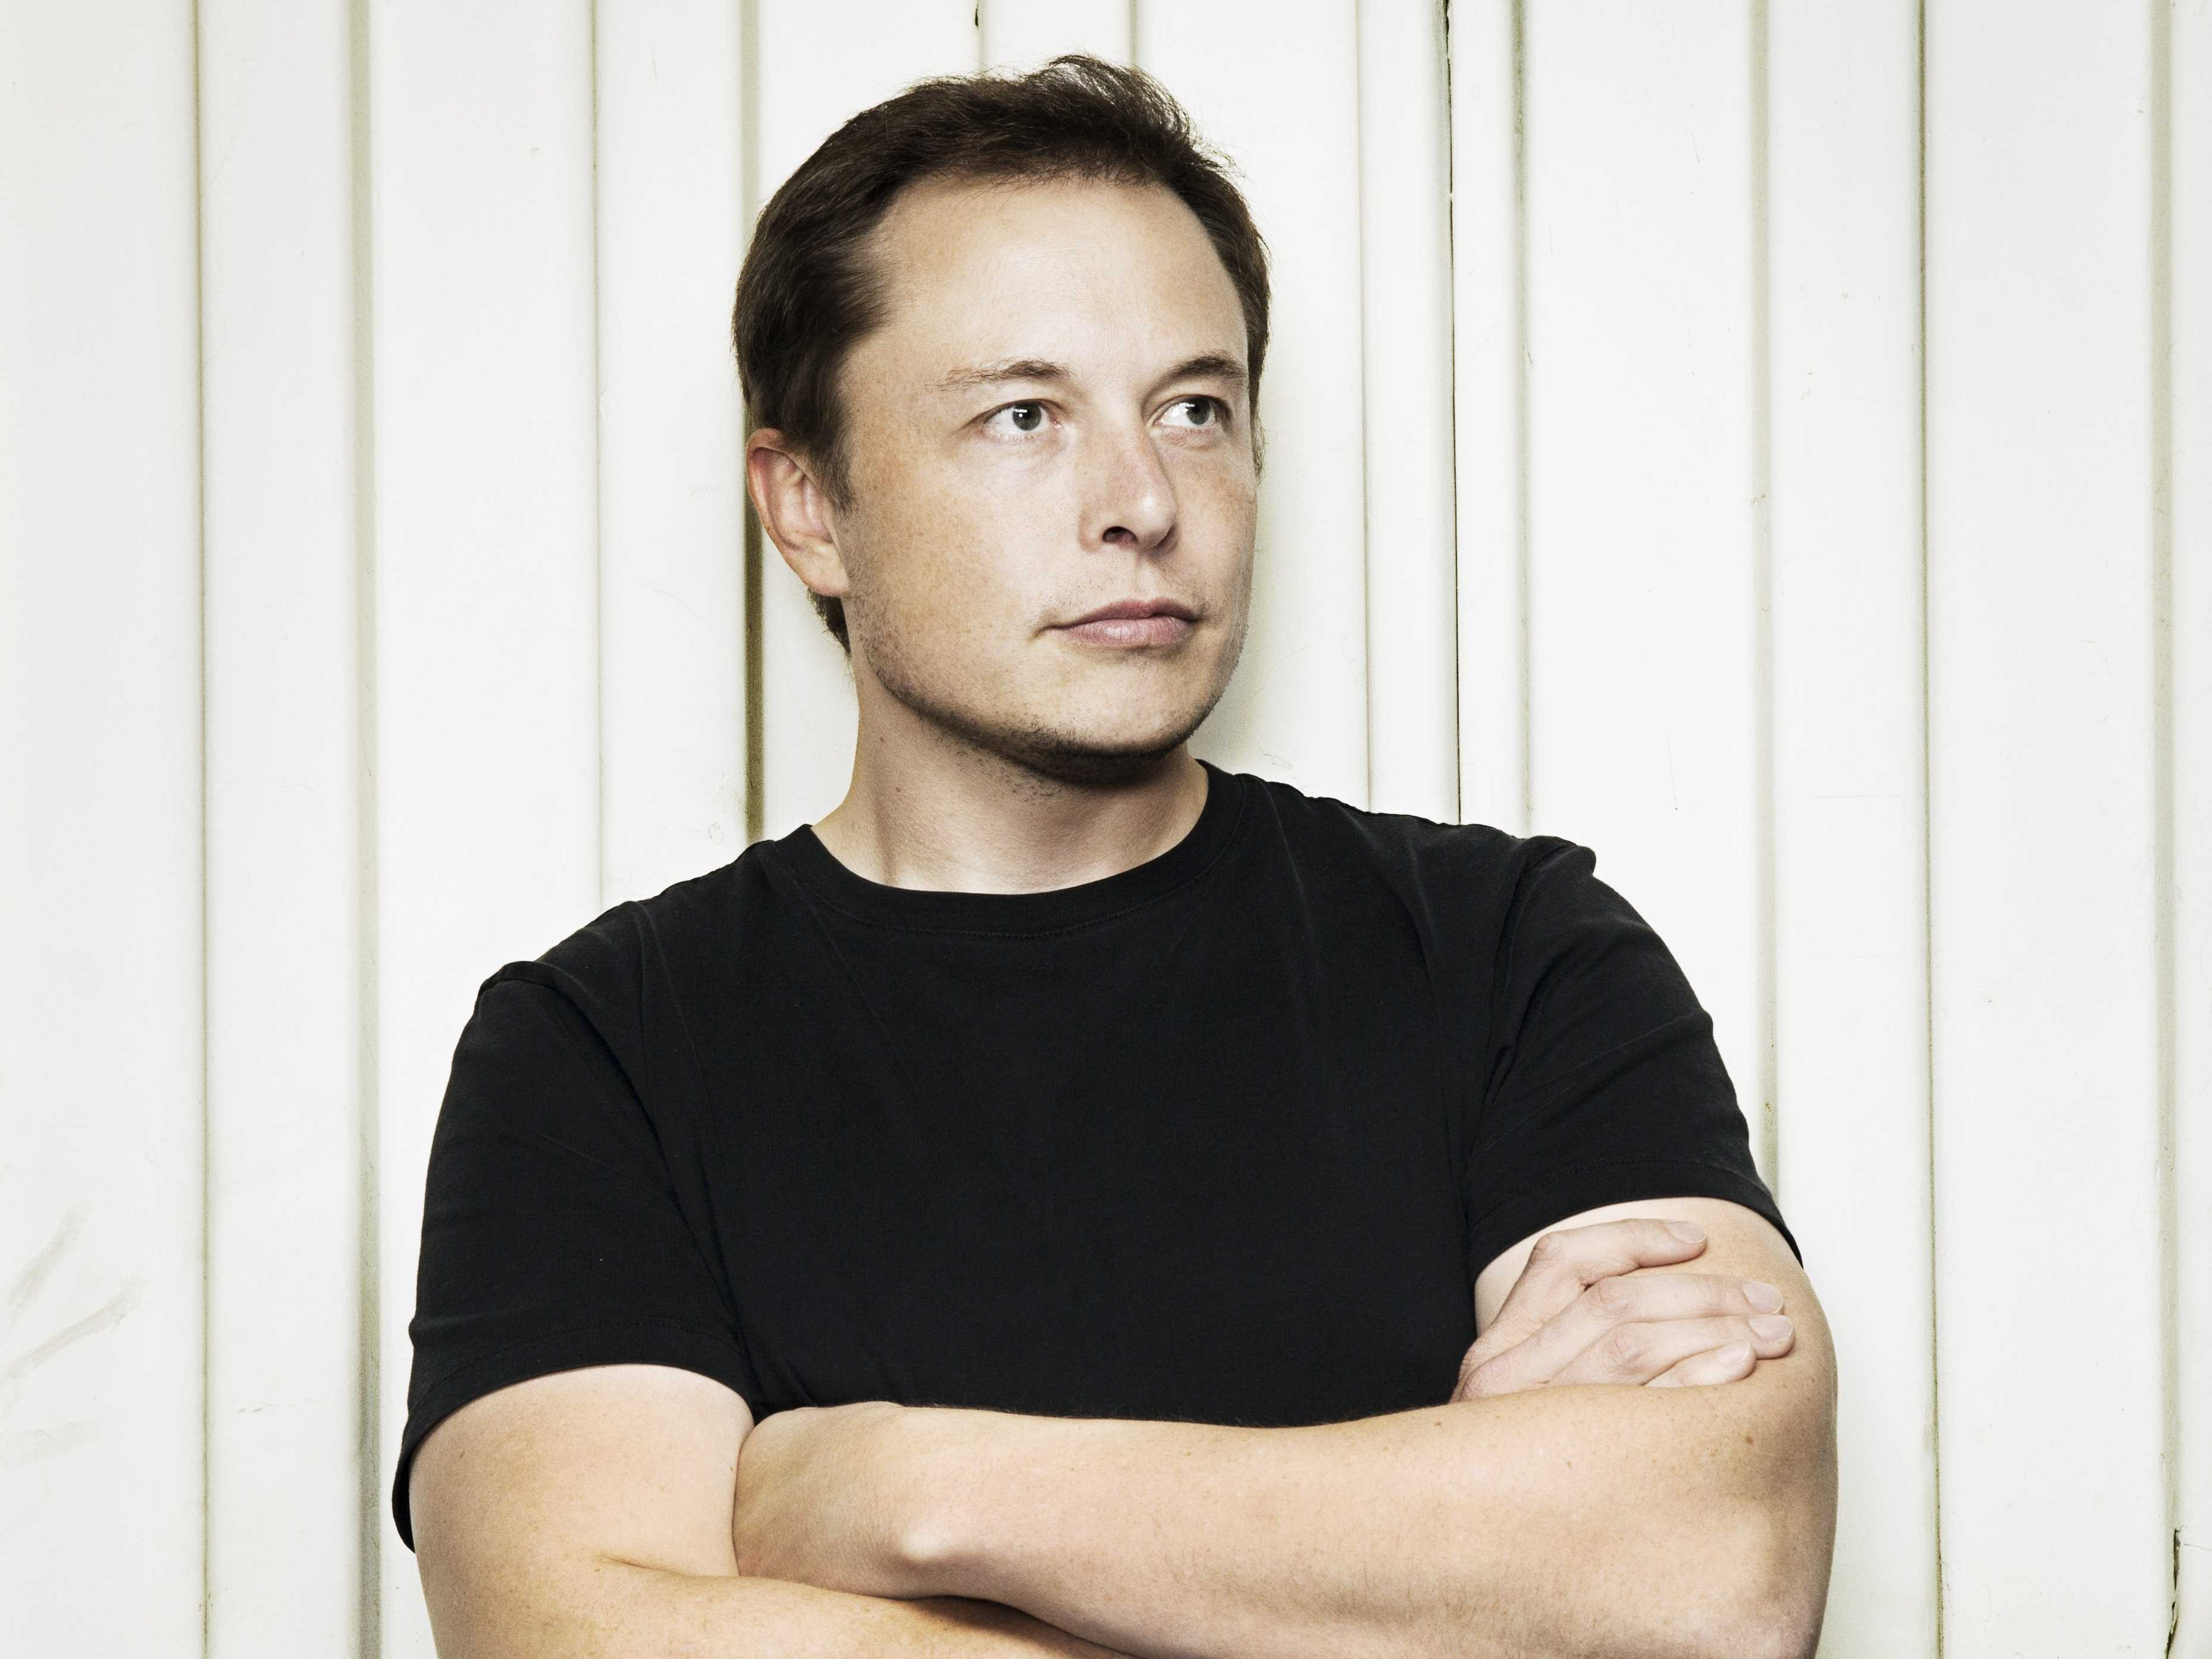
\includegraphics[width=45mm]{images/musk.jpg}
        \end{column}
    \end{columns}
    \item Does not want to die on Earth
\end{itemize}
\end{frame}


\subsection{Carrier}
\begin{frame}
\frametitle{Carrier}
\begin{itemize}
    \itemsep1em
    \item Zip2, co-founded in 1995
    \item Paypal, co-founded in 1999
    \item CEO and CTO of SpaceX, founded in 2001
    \item CEO and CTO of Tesla Motors, founded in 2003
    \item Chairman of SolarCity, founded in 2006
    \item Hyperloop, concept created in 2014
    \item Co-chairman of OpenAI, co-founded in 2015
\end{itemize}
\end{frame}


\subsection{Long term goals}
\begin{frame}
\frametitle{Long term goals}
\begin{itemize}
    \itemsep1.5em
    \item Breaking the legacies of transportation technologies
    \item Traveling on Mars
    \item Stop using fossil fuels as our main power source
    \item Avoid the humanity to die before the next 2 centuries
\end{itemize}
\end{frame}


\begin{frame}
\frametitle{Transportation technologies}
\begin{itemize}
    \itemsep1em
    \item Electric cars with Tesla Motors
    \item Add a transportation system between trains and planes, with the
        Hyperloop
    \item Reusable rockets, able to land, because:
        \begin{quote}
            ``Obviously it'd be kind of weird if the aliens landed in the ocean
            with parachutes, we'd be like okay, nothing to fear.'' Elon Musk to
            a journalist.
        \end{quote}
\end{itemize}
\end{frame}

    \section{Inspired by the Ford's strategies}

\subsection{A little bit of history}
\begin{frame}
\frametitle{A little bit of history}
\begin{itemize}
    \itemsep1em
    \item Cars were electrics in 1903
    \item Ford needed to reduce the production costs of thermal engines
    \item Developing a new way to produce faster
    \item Seems to have worked since 1908 and the Ford T
    \item Product advertisement was not needed between 1917 and 1923
\end{itemize}
\end{frame}

\subsection{Electric cars}
\begin{frame}
\frametitle{No one wants electric cars to be on the market}
\begin{itemize}
    \itemsep1.5em
    \item Selling classic cars would be difficult
    \item Requires investments
    \item Lobbying by the oil industry
    \item Governments are not pushing it enough
\end{itemize}
\end{frame}

\begin{frame}
\frametitle{Everyone wants an electric car}
\begin{itemize}
    \itemsep1.5em
    \item Smooth feeling on the road
    \item Decrease the dependency to oil
    \item Reduces the pollution released compares to classic cars
    \item Everybody seems to agree it is the future car
\end{itemize}
\end{frame}

\begin{frame}
\frametitle{But…}
\begin{itemize}
    \itemsep1.5em
    \item What about the autonomy?
    \item The drive might be slow… no?
    \item Reducing the pollution… really?
    \item OK but… it has to be today? Not… like… tomorrow?
\end{itemize}
\end{frame}


\subsection{Space travels}

\begin{frame}
\frametitle{Space travels}
\begin{itemize}
    \itemsep1.5em
    \item Technology issues
    \item High costs
\end{itemize}
\end{frame}


\end{document}
